\section{Recherche}

Im Zuge unserer Recherche haben wir beschlossen, uns grob an einem Plan von Nick Roethe für einen \glqq{}80m-1W-Fuchsjagdsender\grqq{} für unseren Aufbau zu orientieren.\\
\begin{figure}[H]
	\centering
	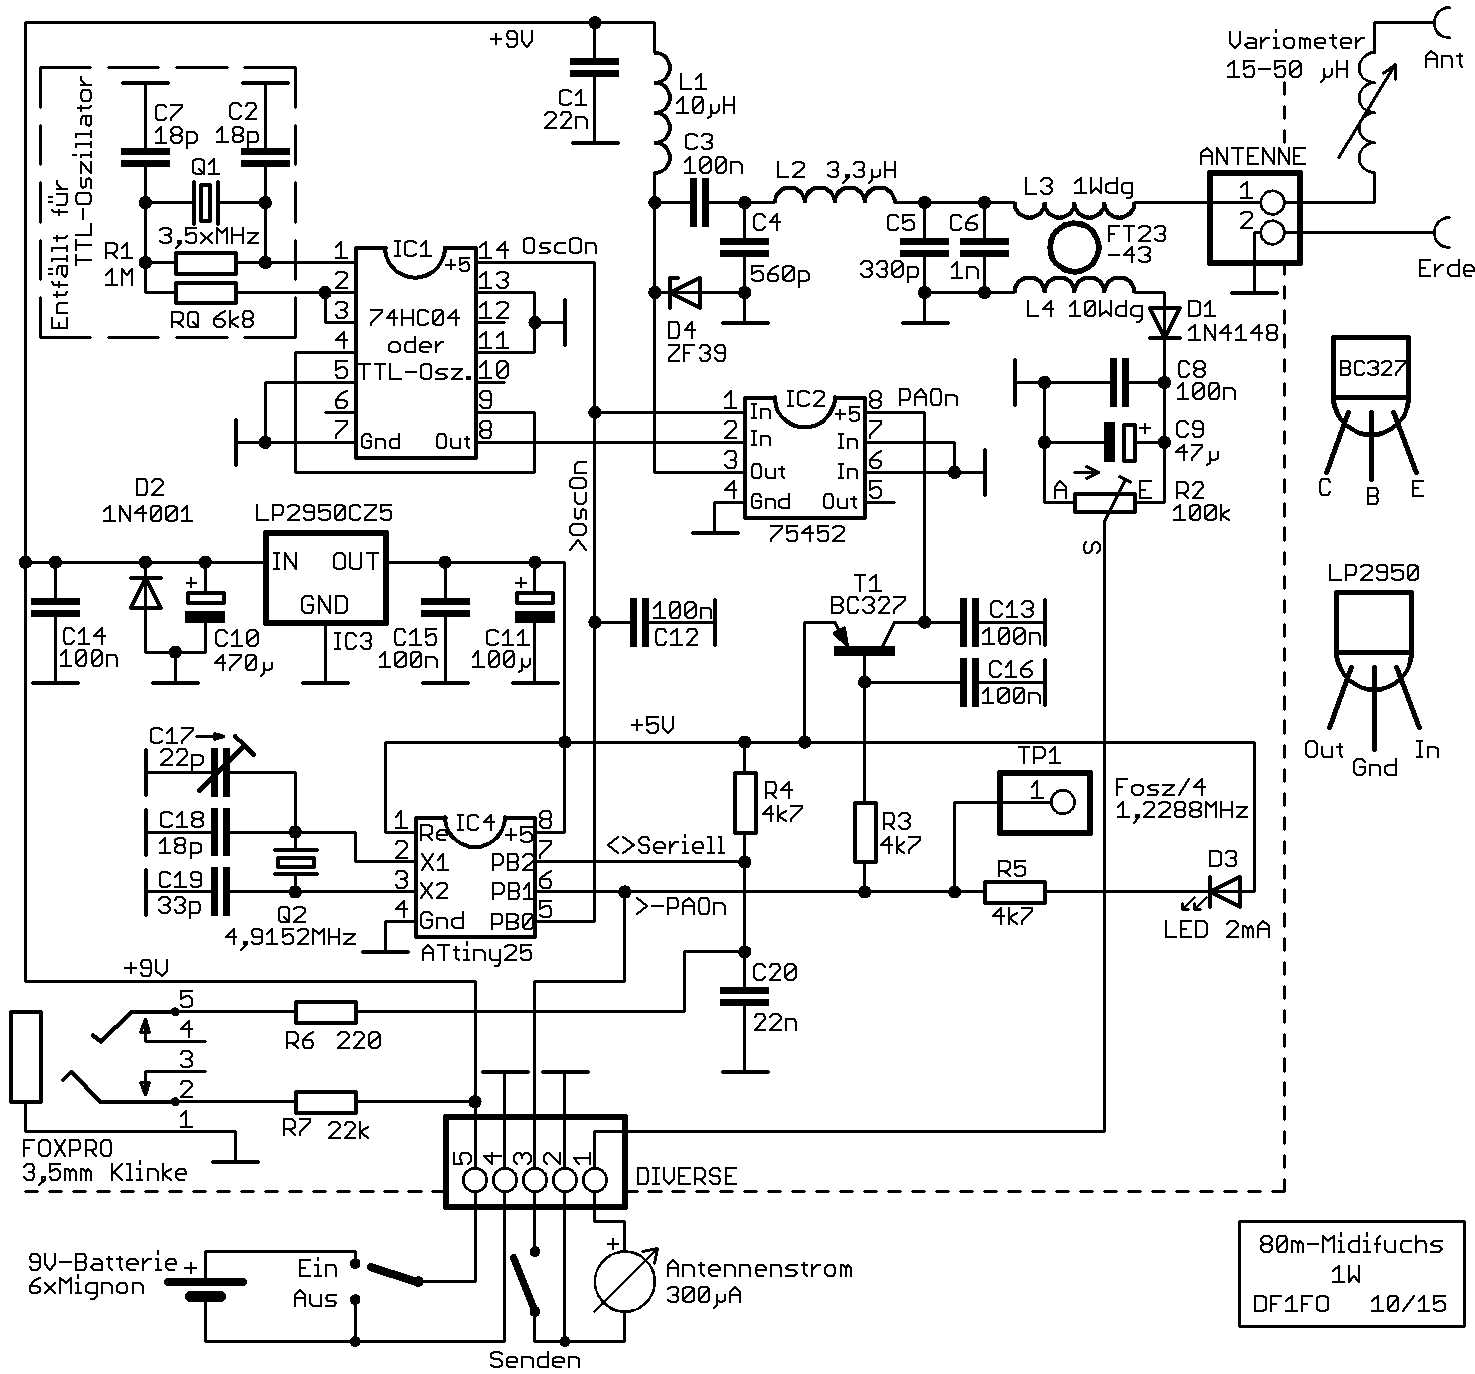
\includegraphics[width=16cm]{res/Recherche_Aufbau.png}
	\caption{Schaltung des Fuchsjagdsenders von Nick Roethe}
\end{figure}

Für die Wahl unserer Bauteile haben wir uns wo möglich für SMD-Bauteile entschieden wegen der kleineren Serieninduktivität der Kondensatoren und zur Platzersparnis.
Indem wir für die Bedienung ein Potentiometer verwenden, das wir mit Hilfe eines DIP-Schalters umschalten können wir am Mikrocontroller I/O-Pins sparen und so bei einem billigeren Modell bleiben. 
Um die Anforderungen bezüglich der Energieversorgung zu erfüllen sollten 3 Lithium-Polymer-Zellen mehr als ausreichen.

%toDo: Fällt noch wem was ein?
